\section{Background}

%We first describe an example Best Practice Guidelines (\BPG{}) to
%explain characteristics that a \CIG{} language needs to have. We then
%explain limitations in existing approaches, and introduce our
%\emph{semantics-first} methodology.

We first introduce relevant background work before discussing research challenges.
In section \ref{subsec:cdss}, a real-world \BPG{} for management of sepsis
in pediatric cases is used to introduce Guidelines-based \CDSSs{} and illustrate
characteristics desirable of a framework for building \CDSSs{}.
In section \ref{subsec:related-work}, we desribe progress
made towards addressing said challenges by existing approaches and their limitations.
Central to our approach is the \emph{semantics-first} philosophy,
which is introduced in section \ref{subsec:semantics-first}.
Section \ref{subsec:medik} introduces the \MediK{} \DSL{} for
\emph{executable} \BPGs{} and explains how its design satisfies aforementioned
characteristics. Section \ref{subsec:sepsis-cdss} discusses the \MediK{}-based
\emph{executable} \BPG{} for management of sepsis and the corresponding \CDSS{}.

\subsection{Guidelines-based Clinical Decision Support Systems}\label{subsec:cdss}

We use a real-world \BPG{} for management of sepsis
in pediatric cases used at the Children's Hospital of Illinois at OSF St.
Francis Medical Center (OSF) to introduce \BPGs{} and Guidelines-based Clinical Decision
Support Systems (\CDSSs{}), and illustrate characteristics desirable of a framework for such system.
Sepsis is life-threatening condition caused by the body's extreme response to
an infection \cite{RhodesICM17}, and is
a major cause of morbidity and mortality in children \cite{Eisenberg2021JP}.
Adverse outcomes can, however, be mitigated through timely
identification and prompt treatment with antibiotics and
intravenous (IV) fluids \cite{Weiss2014CCM,Evans2018JAMA}.
\BPGs{} for screening and management of sepsis in pediatric Emergency
Departments (EDs) have shown effectiveness in screening and management of sepsis \cite{Eisenberg2021JP},
leading to their adoption in many pediatric EDs \cite{Balamuth2017EM,Sepanski2014FP}.

\begin{figure}
  \begin{subfigure}[b]{0.5\textwidth}
    \centering
    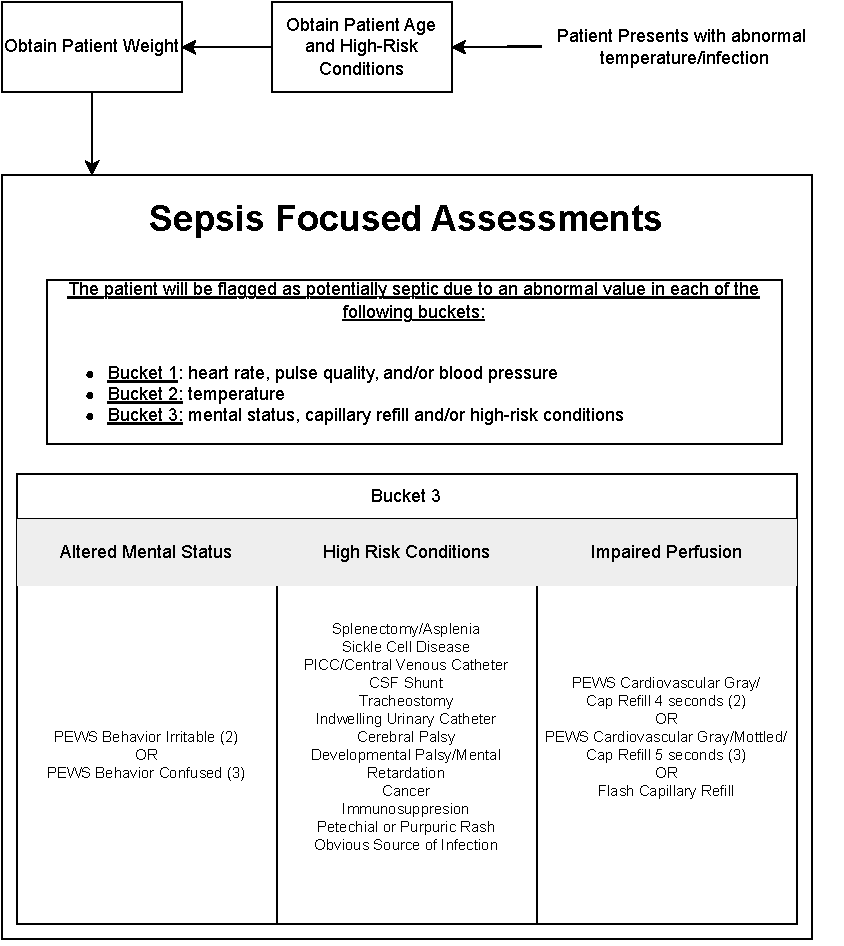
\includegraphics[width=0.65\textwidth]{sepsis-screening-osf}
    %\includegraphics[width=0.5\textwidth]{screening-vitals}
    \caption{Pediatric sepsis screening \BPG{}}\label{fig:sepsis-screening}
  \end{subfigure}
  \begin{subfigure}[b]{0.3\textwidth}
    \tiny
      \begin{tabular}{ | c || c | c | c | }
        \hline
        \textbf{Age}            & \textbf{Heart Rate}   & \textbf{Systolic BP} & \textbf{Temp}  \\
        \hline
        $0d - 1m$               & $>205$                & $<60$                & $<36 \text{ or } >38$ \\
        \hline
        $\geq 1m - 3m$          & $>205$                & $<70$                & $<36 \text{ or } >38$ \\
        \hline
        $\geq 3m - 1y$          & $>190$                & $<70$                & $<36 \text{ or } >38.5$ \\
        \hline
        $\dots$                 & $\dots$               & $\dots$              & $\dots$ \\
        \hline
        $\geq 13y$              & $>100$                & $<90$                & $<36 \text{ or } >38.5$ \\
        \hline
      \end{tabular}
      \caption{Vital Signs Chart}\label{table:vital-signs}
  \end{subfigure}
\end{figure}

In \figurename{} \ref{fig:sepsis-screening}, we present a simplified version of
the screening section of OSF's sepsis management guideline.
In essence, when a patient arrives at the
\ED{} with a fever or an infection, the \HCP{} is supposed to obtain
\begin{enumerate*}[label=(\alph*)]
  \item the patient's age,
  \item any conditions, such as cancer, immunosuppresssion, etc,
    that increase likelihood of sepsis, and
  \item the patient's vital signs, such as heart rate, systolic blood
    pressure, respiratory rate, etc.
\end{enumerate*}
This information is then used to check for abnormalities
in clusters of linked information, called \say{buckets}. For instance, if
the patient's heart rate is abnormal, then \say{bucket 1} is said to
have an abnormal value.
Checking for such abnormalities often involves the use of tables, such as
\tablename{} \ref{table:vital-signs}, that contain normal ranges indexed by
\emph{age}.
%\footnote{For brevity, we omit some age ranges and vital signs from table
%\ref{table:vital-signs}}.
If the patient has at least one abnormal value in every \say{bucket},
then he/she is flagged as potentially septic.

The \BPG{}-recommended treatment for
sepsis involves multiple concurrent workflows, such as
screening for septic shock, fluid resuscitation, and administering antibiotics.
In \figurename{} \ref{fig:fluid-therapy}, we provide
a version of the fluid resuscitation guideline used
at OSF. Briefly, if the patient is flagged as potentially septic, the guideline suggests
\begin{enumerate*}[label=(\roman*)]
  \item obtaining any fluid-overload risks,
  \item administering normal saline (typically over a period of 15 minutes),
    where the dosage is dictated by risks determined in previous step,
  \item assessing signs of fluid-overload,
  \item evaluating patient responsiveness to normal saline upon completion of
    the administering process, and,
  \item determining whether another fluid bolus should be administered based on
    information from previous steps.
\end{enumerate*}
\begin{figure}[b]
  \centering
  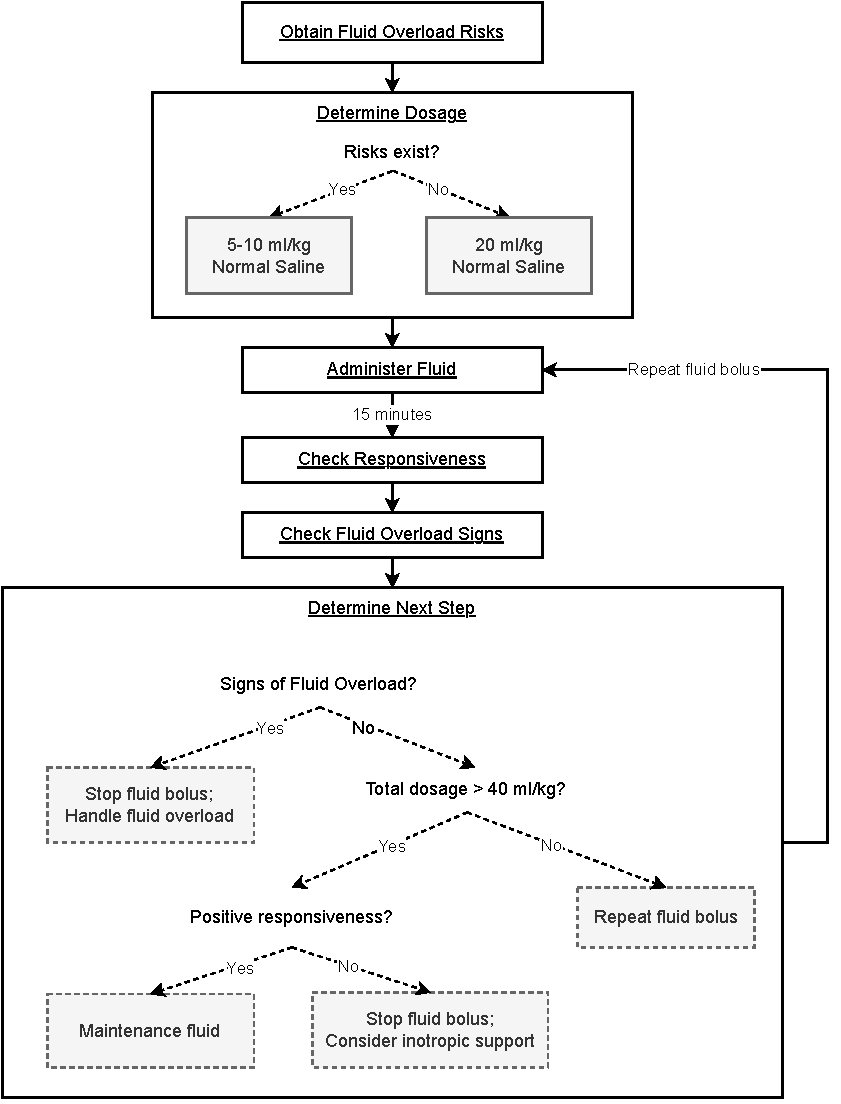
\includegraphics[scale=0.45]{FluidWorkflow-fmcad.pdf}
  \caption{Fluid Resuscitation Guideline}\label{fig:fluid-therapy}
\end{figure}

This real-world \BPG{} exhibits characteristics common
across many \BPGs{}. Specifically \BPGs{} typically:
\begin{itemize}
  \item Involve \stress{concurrent} workflows, such as administering drugs,
    monitoring vitals, performing treatment, etc. There may also be
    inter-workflow interactions. For instance, a diagnosis of sepsis during the
    screening may require modifications to an ongoing course antibiotics.
  \item Often specified in a \stress{flowchart-like}
    notation. See \cite{AHAFlowcharts} and \cite{CancerCareFlowcharts} for other flowchart-based \BPGs{} for management of \emph{cardiac arrest}, and
    screening, risk-reduction, treatment and survivorship in
    cancer care respectively.
  \item Require communication between \stress{heterogeneous agents} such as
     monitors and Electronic Health Records (EHRs).
  \item Often use \stress{tables} indexed by parameters such as age, weight,
    etc to present normal/abnormal ranges for measurements, or recommended dosages for drugs.
\end{itemize}

%\begin{center}
%\renewcommand{\arraystretch}{0.5}
%\setlength\extrarowheight{-9pt}
  \begin{table}
    \tiny
  \begin{tabularx}{\textwidth}{
      >{\centering\arraybackslash}X
    || >{\centering\arraybackslash}X
    | >{\centering\arraybackslash}X
    | >{\centering\arraybackslash}X
    | >{\centering\arraybackslash}X
    | >{\centering\arraybackslash}X
  }
                 & Specification-Implementation Gap  & Complex Workflows  & Diverse Agents   & Formal Analysis  & Holistic Safety  \\
    Arden Syntax & $\greencheck$                     & $\redcross$        & $\redcross$    & $\redcross$        & $\redcross$ \\
    GLIF         & $\greencheck$                     & $\greencheck$      & $\redcross$    & $\redcross$        & $\redcross$ \\
    Asbru        & $\greencheck$                     & $\greencheck$      & $\redcross$    & $\greencheck$      & $\redcross$ \\
    PROForma     & $\greencheck$                     & $\greencheck$      & $\redcross$    & $\redcross$        & $\redcross$ \\
    GLARE        & $\greencheck$                     & $\greencheck$      & $\redcross$    & $\cancelcheck$     & $\cancelcheck$ \\
    SAGE         & $\greencheck$                     & $\greencheck$      & $\greencheck$  & $\redcross$        & $\redcross$ \\
    Promela/SPIN & $\redcross$                       & $\greencheck$      & $\redcross$    & $\greencheck$      & $\cancelcheck$ \\
    AMSs         & $\redcross$                       & $\greencheck$      & $\redcross$    & $\greencheck$      & $\redcross$ \\
    P            & $\redcross$                       & $\greencheck$      & $\greencheck$  & $\greencheck$      & $\redcross$ \\
  \end{tabularx}
  \caption{Comparison of Existing Approaches}\label{table:existing-approaches}
  \end{table}
%\end{center}

\subsection{Related Work}\label{subsec:related-work}

Recall from section \ref{sec:introduction} the following
challenges in building \CDSSs{}:
\begin{itemize}
  \item \textbf{Specification-Implementation Gap:} The specification,
    i.e., the \BPG{}, may differ from its translation in a computable
    medium, i.e. \CIG{}.
  \item \textbf{Complexity:} \BPGs{} encode complex medical knowledge,
    involving multiple \emph{concurrent} workflows and \emph{inter-workflow}
    interactions. Moroever, $\CDSSs{}$ interact with \emph{diverse
    external agents} such as medical sensors and patient records.
  \item \textbf{Formal Analysis:} As \CDSSs{} are \emph{safety-critical},
    it's desirable to have execution engines with \emph{correctness guarantees}
    and a suite of formal analysis tools such as model checkers and deductive
    verifiers that can handle aforementioned complexity.
  \item \textbf{Holistic Safety:} A mechanism for establishing the safety
    of the entire system must exist. This includes reasoning about external
    components, and safely integrating AI-enabled components.
\end{itemize}

Existing research has been instrumental in both recognizing aforementioned
challenges and adressing them to various degrees, leading to greater \CDSS{}
adoption. In \tablename{} \ref{table:existing-approaches}, we provide an overview of
how existing work addresses aforementioned challenges. We use
\greencheck{}, \cancelcheck{}, and \redcross{} to depict that an approach
fully-addresses, partly-addresses, or doesn't address a limitation respectively.
We next go over notable approaches, and describe how they incrementally
address said challenges.

\paragraph{Arden Syntax:}

The Arden Syntax \cite{HripcsakCBM94} is a widely used medium for
writing executable \BPGs{}. First proposed in 1989, it was among the
first languages to recognize and address the \emph{specification-implementation
gap} by emphasizing \emph{comprehensibility} to non-experts in Computer Science \cite{SamwaldJBI12}.
Guidelines are described using Medical
Logic Modules that contains information related to guideline's purpose
, maintenance, and medical knowledge. The modules are modular to allow
re-use and sharing across hospitals. But, Arden Syntax
is focused on describing simple, modular, and independent
guidelines (such as reminders), and not on guidelines with complex logic (such
as treatment protocols) \cite{PelegJBI01}.

\paragraph{GLIF:}

Arden Syntax's limitation in modeling complexity is addressed by
GLIF \cite{BoxwalaJBI04}: a language that uses flowcharts to expressed
guidelines. A multi-level approach is
employed to manage complexity: at the top is the conceptual level, where
only high-level details relevant for human-comprehension are present. In the
middle is a computable-level, where details of guideline execution flow
and patient data elements are specified. At the bottom is the implementable
level, where institution-specific details and mappings into patient data are
specified. Both Arden Syntax and GLIF  eliminate
the gap between the \BPG{}, i.e. the specification, and the \CIG{}, i.e. implementation as
they're meant to be either directly used by clinicians (or in collaboration with
computer scientists) to express \BPGs{} in an executable medium. \CIGs{}
expressed in them are meant to be shared across hospitals, and are thus modular.
However, neither formalism has complete formal semantics, or comprehensive support for
rigorous formal analysis.

\paragraph{Asbru:}

The need for formal analysis is identified by Asbru: a formalism with formally
defined syntax and semantics \cite{ShaharAMIA96}. In Asbru, a guideline is modeled as a plan
that contains:
\begin{enumerate*}[label=(\roman*)]
  \item intentions that define aims,
  \item conditions that specify when the plan is applicable,
  \item effects that define expected behavior during execution, and,
  \item a body containing other subplans.
\end{enumerate*}
Apart from an execution engine, the Asbru ecosystem also contains
other tools, such as a model checker for verification \cite{BaumlerSPIN06}.
However, the formal semantics of Asbru have been only partially defined, and
is insufficient to implement tools for the language \cite{SuttonAMIA03}.

\paragraph{PROForma:}

The importance of a complete formal-semantics is identified and addressed
by PROforma \cite{SuttonAMIA03}, another formalism that uses plans to
model guidelines. A PROforma plan is made of a sequence of tasks.
The plan defines constraints on their enactment, and circumstances
for termination (for example, exceptions) \cite{SuttonAMIA03}. But, despite
having complete formal semantics, it does not have a comprehensive suite of
formal analysis tools such as model checkers, deductive verifiers.

\paragraph{SAGE:}
The SAGE guideline model \cite{TuSAGE04} uses the Prot\'eg\'e knowledge
representation framework \cite{NoyAMIA03} to model guidelines,
and improves on aforementioned approaches by
enabling seamless integration into hospitals' existing Clinical Information Systems
(\CISs). But, it lacks complete formal semantics, and analysis tools
such as deductive verifiers and model checkers.
The GLARE formalism \cite{TerenzianiBook04} uses an actions based approach
to represent guidelines, and addresses clinician-comprehensibility and
modularity. For formal analysis, GLARE guidelines can be translated to
Promela: the SPIN model checker's specification language \cite{GiordanoAMIA06}.
The approach partly addresses holistic safety as
external agents (such as clinicians) can be modelled and analyzed.
But, the scenario where the external agent's behavior
deviates from the model during system execution isn't addressed.


Languages outside the medical domain can also be used to reason about
medical systems. For example, in \cite{ArcainiMEMCODE15}, Abstract State
Machines (\ASMs) are used to validate and verify a system for measuring
patients' stereoacuity in the diagnosis of amyblyopia.
Along similar lines, the P language \cite{DesaiPLDI13}
and analysis of large concurrent systems provides a convenient medium
for expressing multiple workflows and interactions as concurrently
executing Finite State Machines (FSMs). External agents can be modeled
using \emph{ghost} that are used for formal analysis, but discarded at runtime.
But such formalisms, while suitable for formal verification, may
not be easily comprehensible to clinicians for validation.

This proposal aim to build on progress made by existing work to comprehensively
address all challenges mentioned earlier. Next, we describe the
\emph{semantics-first} approach to building systems.

\subsection{Semantics-First Approach}\label{subsec:semantics-first}

The semantics first approach dictates that the semantics
of a language should be formally defined. Tools for the language
such as interpreters, compilers, model checkers and deductive
verifiers should be derived from the semantics in a
\emph{correct-by-construction} fashion, instead of being implemented
from scratch in an ad-hoc manner.

For a language like \MediK{}, the semantics first approach has many benefits. First,
since \MediK{} is meant to be used in safety-critical settings,
it's vital that its interpreter has correctness guarantees, which
the approach ensures. Second, \MediK{} has to evolve quickly
to incorporate feedback that it receives from domain experts.
Such changes in the semantics-first approach only require changes to
the semantics, and all tools are updated automatically.

\subsection{\MediK{}}\label{subsec:medik}
Here we discuss sepsis guideline in \MediK{}


\subsection{Pediatric Sepsis Executable \BPG{}}\label{subsec:sepsis-cdss}
Pediatric sepsis \CDSS{} in \MediK{}


